\section{Introduction}

\subsection{Overview}

As the population increases the traffic management is becoming more complex and challenging in various urban areas around the world.  This high demand of traffic management required a modelling, simulation and observation of the traffic flow and being able to monitor the effect of traffic congestion and incidences to study the effectiveness of the signs, hardware devices such as traffic lights and other barriers that are used to manage and improve the traffic policies and guild-lines related to the traffic management regulation, and also being able to assist the design and development of roads, junctions and highways.\newline

One of the effective tools used in order to overcome the high demand of population and being able to analyse a wide range of dynamic problem associated with complex scenarios which cannot be described in an analytical approach is simulation modelling. These simulating models have been classified by the level of detailing and its interaction based on various system entities or component, which there interaction are complex in real world. these simulations models represent the dynamic behaviour in a mathematical and logical way in the system operation. Over the past six decades there has been significant improvement in design and development of the traffic simulation models in order to experiment the real world traffic operation there are various techniques and approaches used in implementation and design of these simulation models which   now days the use of these tool are necessary in order to analyse and examine the real world scenario of the traffic operation, which is a common tool used for traffic engineers. The following list are the main reason for the need of traffic simulation:

\begin{enumerate}
\item When we require to observe the behaviour of the vehicles and entitles of the system such as traffic signs and traffic lights in an animated way.
\item When there is an uncertainty in the mathematical analysis result.  
\item In instances where the analytical or mathematical modelling approach is inadequate or infeasible, this can be due to the complexity of the urban operation.
\end{enumerate}

In this project we have designed and developed a traffic simulation by animating the vehicle operation on a 2-Dimention map as shown in figure 1, where the vehicles can operate on single and multi-lane, on opposite directions. Our approach adapts the agent based-method where the vehicle detect their condition based on their position where the vehicle can stop or turn depending on their position. The user has the ability to change the parameters of the system such increasing and decreasing the numbers of cars, delay of the traffic light and flow-rate (frequency). The user has various map selection as shown, this can be either a single junction or multiple junction operation and the user has the ability to change the delay of the traffic light. In this project we have considered and adapted the traffic policies, such as implementing traffic lights in order to manage the traffic flow and designed various lanes and junction considering the road network operation. The system has a time control follow density operation, where the number of cars operating in the system increases to it maximum limit   as the time merges its peak time. \newline

\begin{figure}[H]
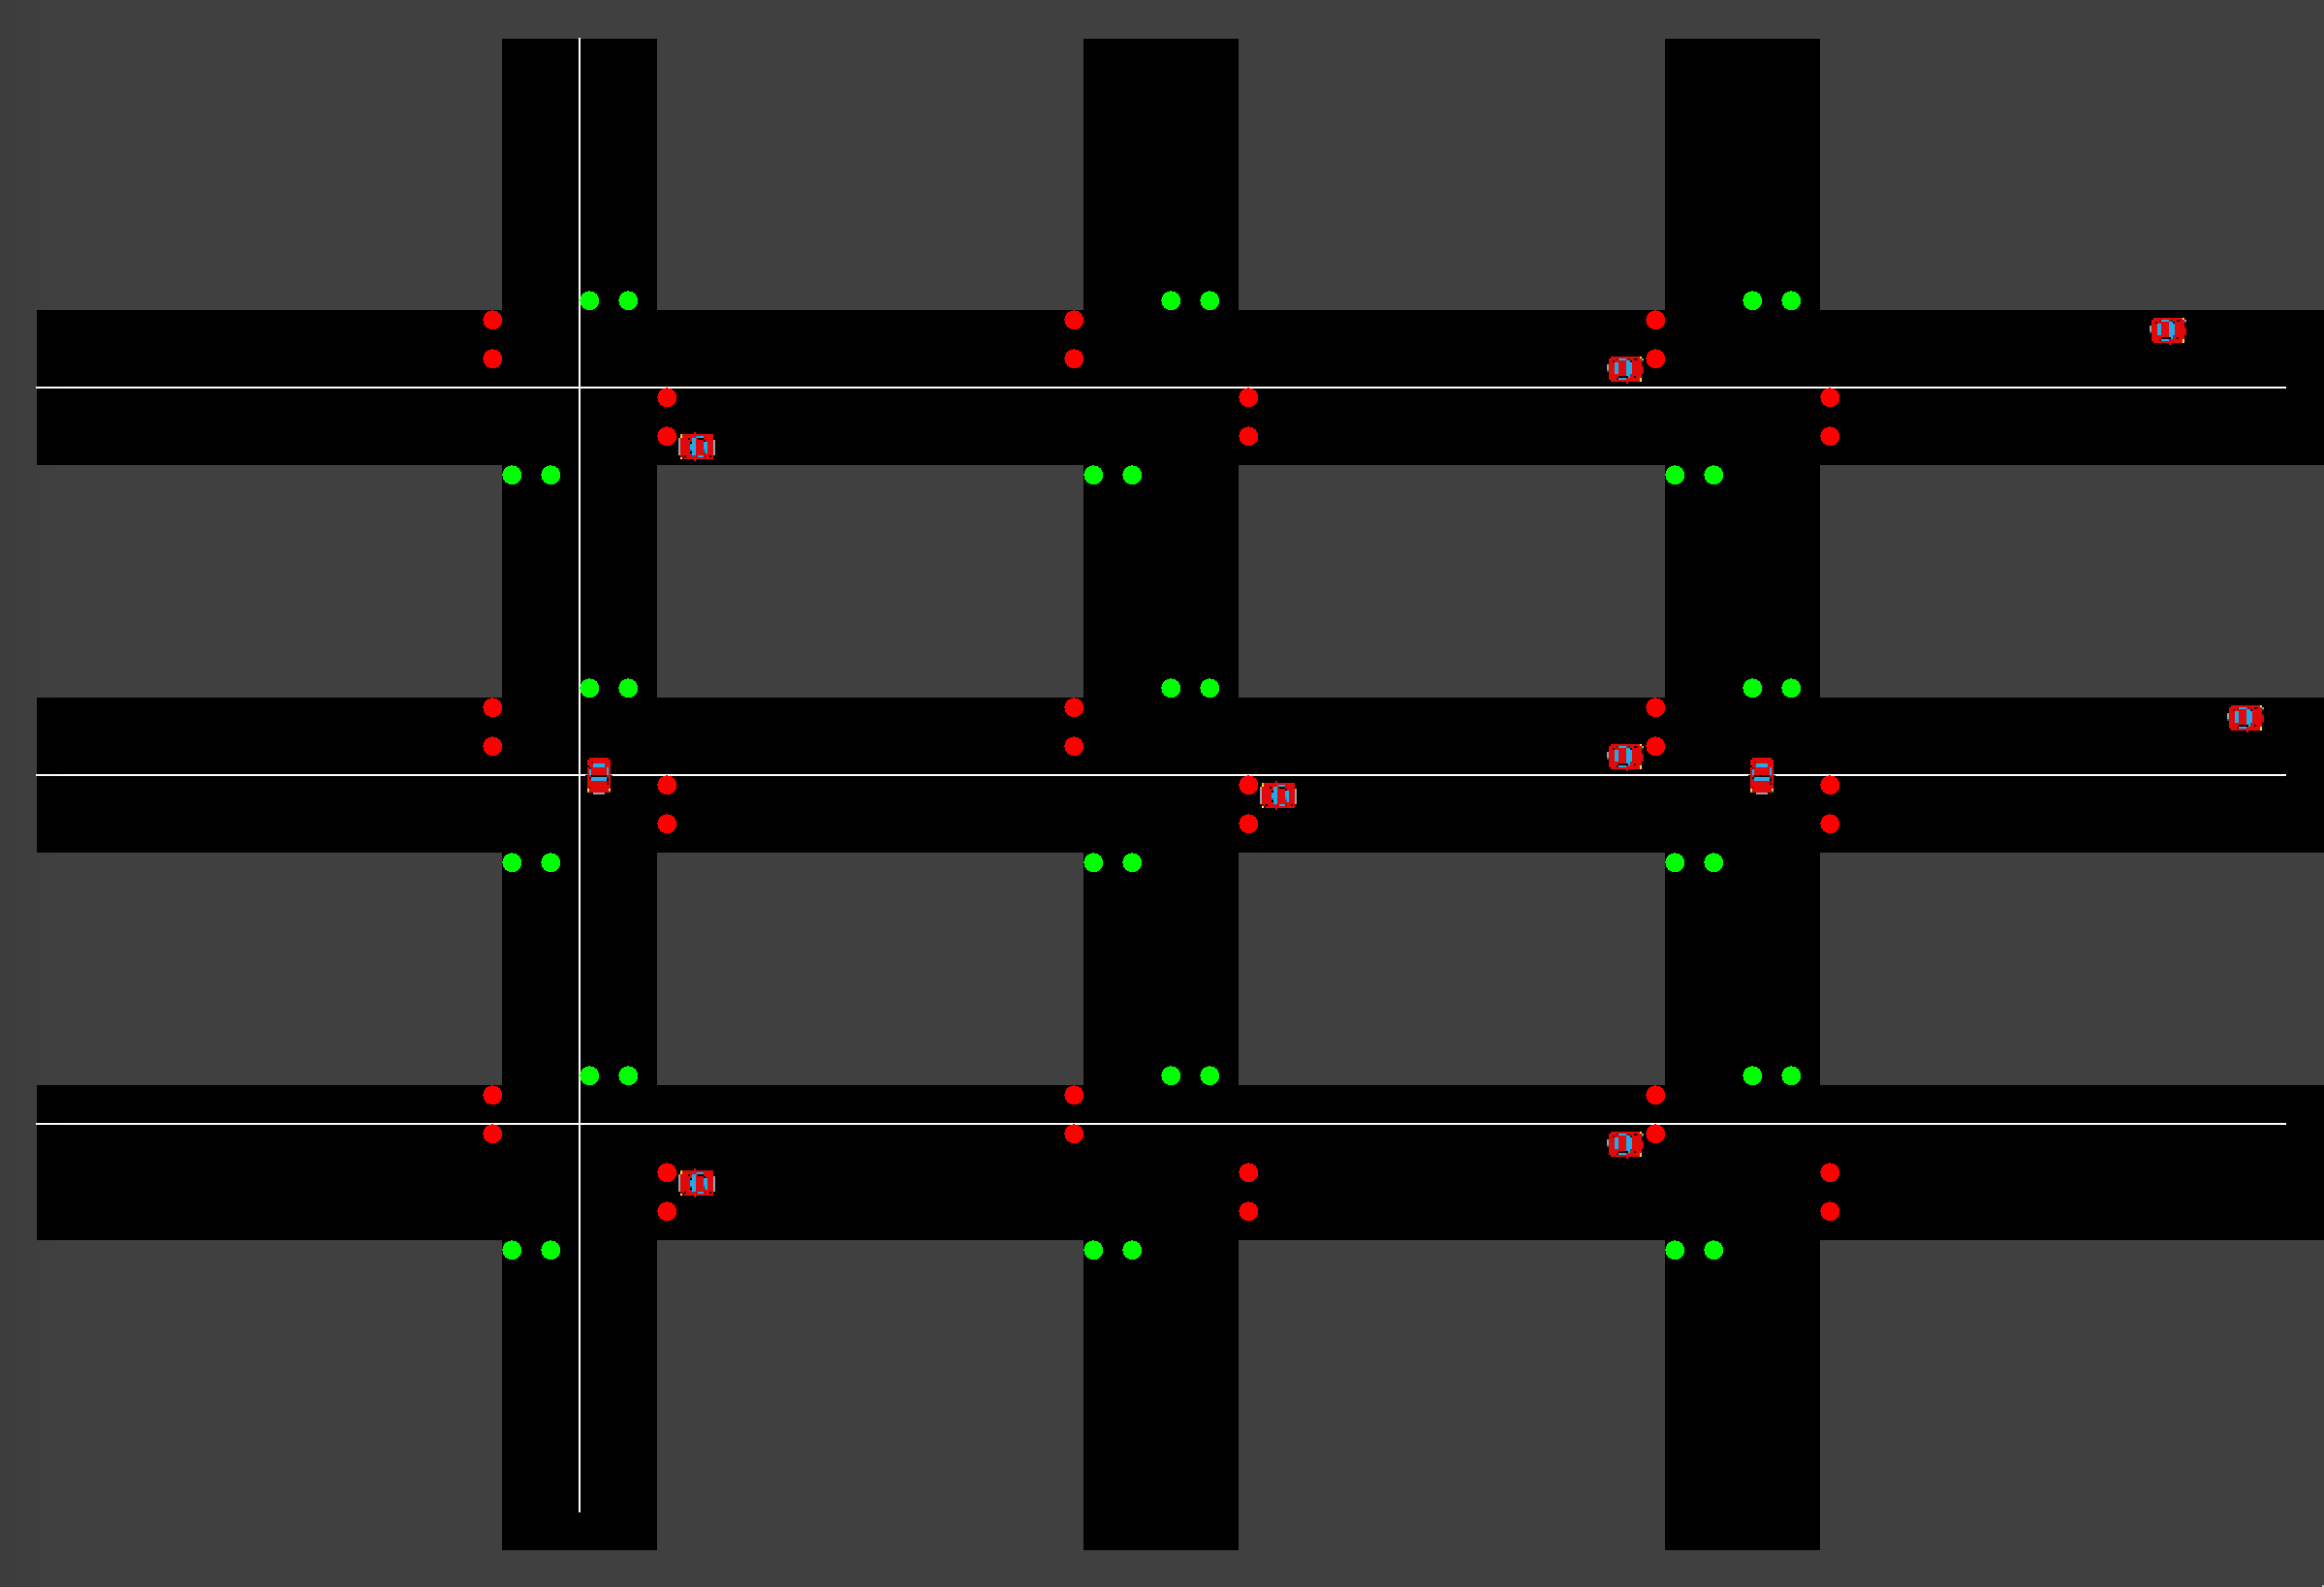
\includegraphics[width=12cm, height=12cm]{pics/trafficSimu}
\centering
\caption{Map bird-eye view}
\end{figure}

\subsection{Aims and objectives}
The over aim of this project is to design traffic simulation engine in order to test the traffic management policy. This project is broken into two section where the first section is the backend structure, which contains the main part of the code as it indicates the functionality of the programme. The second section of the project is the front-end, the main purpose of the Graphical User Interface is to simulate the backend provide user interaction in order to change the parameters. The project has number of objectives to achieve the aims, the following list are the objective to be carried out throughout the project:

\begin{itemize}
\item Research and investigate traffic model and fit it into flexible graphical user interface in order to provide a real life scenario for the user.
\item Setting the aim and the requirements for the implementation.
\item Designing a use-case diagram and class diagram.
\item Design and implement the front-end and the backend of the system.
\item White-box testing the code (should include various testing technique such as unit testing and integration testing techniques).
\item Black-box testing of the system, in order to insure that the requirement are met (this will include functional testing approach).
\item Designing and ind�pendant code.
\end{itemize}

